\documentclass[a4paper,12pt]{jarticle}
\usepackage[dvipdfmx]{graphicx}
\usepackage{amsmath}
\usepackage{subfigure}
\usepackage{comment}
\usepackage{array}

\usepackage{ascmac} %枠つき文章

 
\setlength{\hoffset}{0cm}
\setlength{\oddsidemargin}{-3mm}
\setlength{\evensidemargin}{-3cm}
\setlength{\marginparsep}{0cm}
\setlength{\marginparwidth}{0cm}
\setlength{\textheight}{24.7cm}
\setlength{\textwidth}{17cm}
\setlength{\topmargin}{-45pt}

\renewcommand{\baselinestretch}{1.6}
\renewcommand{\floatpagefraction}{1}
\renewcommand{\topfraction}{1}
\renewcommand{\bottomfraction}{1}
\renewcommand{\textfraction}{0}
\renewcommand{\labelenumi}{(\arabic{enumi})}
%\renewcommand{\figurename}{Fig.} %図をFig.にする


%図のキャプションからコロン:を消す
\makeatletter
\long\def\@makecaption#1#2{% #1=図表番号、#2=キャプション本文
\sbox\@tempboxa{#1. #2}
\ifdim \wd\@tempboxa >\hsize
#1 #2\par 
\else
\hb@xt@\hsize{\hfil\box\@tempboxa\hfil}
\fi}
\makeatother

%auhorを右寄せに
\makeatletter
  \def\@maketitle{%
  \newpage\null
  \vskip 2em%
  \begin{center}%
  \let\footnote\thanks
    {\LARGE \@title \par}%
    \vskip 0em%titleとauthorの間隔
  \end{center}% 追加
    \mbox{}\hfill%% 追加
    {\large
      \lineskip 0.5em%
      \begin{tabular}[t]{c}%
        \@author
      \end{tabular}\par}%
    \vskip 3em%authorとdocumentの間隔
  \begin{center}% 追加
    {\large \@date}%
  \end{center}%
  \par\vskip 0.5em}
\makeatother


\begin{document}
%
\title{\vspace{-30mm} 制御系構成特論~レポート課題2}
\author{\underline{機械知能工学専攻~~16344217~~津上~祐典}}
\date{}
%
\maketitle
%
\vspace{-25mm}
%\parindent = 0pt %すべての段落で字下げをしない
%

%%%%%%%%%%%%%%%%%%%%%%%%%%%%%%
%\section*{\fbox{問題}}
%%%%%%%%%%%%%%%%%%%%%%%%%%%%%%
\begin{itembox}[l]{\Large{課題1.}}
以下のシステム方程式を相似変換し,伝達関数を導出せよ.
  \begin{eqnarray}
   \dot{x}(t)&=&Ax(t)+Bu(t) \\
   y(t)&=&Cx(t)+Du(t)
  \end{eqnarray}
\end{itembox}

\vspace{-10mm}
%%%%%%%%%%%%%%%%%%%%%%%%%%%%%%
\section*{\fbox{解答}}
%%%%%%%%%%%%%%%%%%%%%%%%%%%%%%
$z(t)=Tx(t)$(ただし,$T$は正則行列)とおくと,状態方程式は
%
\begin{eqnarray}
 T^{-1}\dot{z}(t)&=&AT^{-1} z(t)+Bu(t) \nonumber\\
  \dot{z}(t)&=&TAT^{-1}z(t)+TBu(t)
\end{eqnarray}
%
となり,出力方程式は
%
\begin{equation}
 y(t)=CT^{-1}z(t)+Du(t)
\end{equation}
%
となる.
%
初期値を零としラプラス変換すると,状態方程式は
\begin{eqnarray}\label{equ:sys}
 sZ(s)&=&TAT^{-1}Z(s)+TBU(s) \nonumber\\
 Z(s)&=&(sI-TAT^{-1})^{-1}TBU(s)
\end{eqnarray}
となり,出力方程式は
\begin{equation}\label{equ:syu}
 Y(s)=CT^{-1}Z(s)+DU(s)
\end{equation}
となる.ただし,$Y(s)=\mathcal{L}[(t)]~,~U(s)=\mathcal{L}[u(t)]$である.
(\ref{equ:sys})式を(\ref{equ:syu})式に代入すると,
%
\begin{equation}
 Y(s)=\left\{CT^{-1}(sI-TAT^{-1})^{-1}TB+D\right\}U(s)
\end{equation}
%
となる.これより伝達関数$G(s)$は
%
\begin{eqnarray}
 G(s)&=&\frac{Y(s)}{U(s)} \nonumber\\
 &=&CT^{-1}(sI-TAT^{-1})^{-1}TB+D \nonumber\\
 &=&CT^{-1}\left\{T(sI-A)T^{-1}\right\}^{-1}TB+D \nonumber\\
 &=&CT^{-1}T(sI-A)^{-1}T^{-1}TB+D \nonumber\\
 &=&C(sI-A)^{-1}B+D
\end{eqnarray}
%
となる.
%%%%%%%%%%%%%%%%%%%%%%%%%%%%%%
\begin{itembox}[l]{\Large{課題2.}}
伝達関数$G(s)$が
\begin{equation}
 G(s)=\frac{s-a}{(s-a)^2+b^2}
  =\left[
  \begin{array}{rc|r}
  a   &~ b ~&~ 1 \\
   -b &~ a ~&~ 0 \\ \hline
   1  &~ 0 ~&~ 0
  \end{array}
  \right]
\end{equation}
で表され,$x(0)=[0~~-1/b]^{\mathrm{T}}$のとき,入力$u(t)=e^{at}$に対する応答
$y(t)$を求めよ.
\end{itembox}

\vspace{-10mm}
%%%%%%%%%%%%%%%%%%%%%%%%%%%%%%
\section*{\fbox{解答}}
%%%%%%%%%%%%%%%%%%%%%%%%%%%%%%
出力$y(t)$は
\begin{eqnarray}
 y(t)&=&C(sI-A)^{-1}x(0)+C(sI-A)^{-1}BU(s) \nonumber\\
 &=&\left[1~~0\right]
  \left[
\begin{array}{cc}
 s-a &-b\\
 b &s-a
\end{array}
\right]^{-1}\left[
\begin{array}{c}
 0\\
 -1/b
\end{array}
\right]+\left[1~~0\right]
\left[
\begin{array}{cc}
 s-a &-b\\
 b &s-a
\end{array}
\right]^{-1}\left[
\begin{array}{c}
 1\\
 0
\end{array}
\right]\frac{1}{s-a}
\nonumber\\
 &=&
  \frac{1}{(s-a)^2+b^2}
  \left[1~~0\right]\left[
\begin{array}{c}
-1\\
 (a-s)/b 
\end{array}
\right]+ \frac{1}{(s-a)^2+b^2}\left[1~~0\right]
\left[
\begin{array}{cc}
 s-a\\
 -b 
\end{array}
\right]\frac{1}{s-a}\nonumber\\
 &=& \frac{-1}{(s-a)^2+b^2}+ \frac{1}{(s-a)^2+b^2}\nonumber\\
 &=&0
\end{eqnarray}
となる.
%
\begin{figure}[tbp]
 \begin{center}
  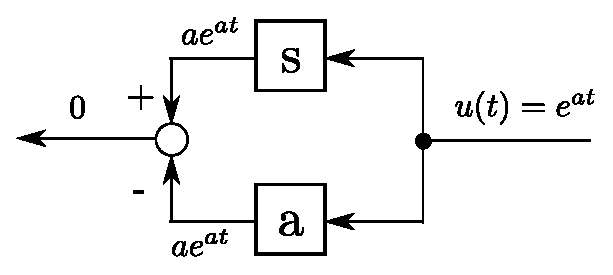
\includegraphics[width=80mm]{fig/burokku.eps}
 \end{center}
 \caption{ブロック線図}
 \label{fig:bro}
\end{figure}
%
$G(s)$の分子に着目したブロック線図を図\ref{fig:bro}に示す.これより入力
$u(t)=e^{at}$が印加されても出力が$0$であることが確認できる.

%%%%%%%%%%%%%%%%%%%%%%%%%%%%%%%%%%%%%%%%
 \begin{itembox}[l]{\Large{課題3.}}
\begin{equation}
 G_1=\frac{s-1}{s+1}~,~G_2=\frac{1}{s-1}
 \end{equation}
 の場合について,直列,並列結合を求め,結合後のシステムの可制御・可観測性
 を調べよ.また,それぞれにおいて,結合後の伝達関数を求めよ.さらに,
 \begin{equation}
  G_1'=G_2'=\frac{1}{s-1}  
 \end{equation}
 のときの並列結合と可制御・可観測性を調べよ.
 \end{itembox}
\vspace{-10mm}
%%%%%%%%%%%%%%%%%%%%%%%%%%%%%%
\section*{\fbox{解答}}
%%%%%%%%%%%%%%%%%%%%%%%%%%%%%%
はじめに$G_1$を厳密なプロパーの形に変換すると,
%
\begin{equation}
 G_1=\frac{s-1}{s+1}=1+\frac{-2}{s+1}
\end{equation}
%
となる.入力を$u$,出力を$y$とすると$y=G_1u$であるから,
%
\begin{eqnarray}
 y&=&\left(1+\frac{-2}{s+1}\right)u \nonumber\\
  &=&-\frac{2}{s+1}u+u
\end{eqnarray}
%
となる.$x$を状態変数とするとシステム方程式は,
%
\begin{eqnarray}
 \dot{x}&=&-x-2u\\
 y&=&x+u
\end{eqnarray}
%
となる.これより伝達関数$G_1$をドイルの記法で記述すると
%
\begin{equation}
 G_1=\left[
  \begin{array}{c|c}
  -1 & -2  \\ \hline
   1 & 1   \\ 
  \end{array}
  \right]
\end{equation}
%
となる.同様に$G_2$をドイルの記法で記述すると
%
\begin{equation}
 G_2=\left[
  \begin{array}{c|c}
  1 ~&~ 1  \\ \hline
  1 ~&~ 0   \\ 
  \end{array}
  \right]
\end{equation}
%
となる.$G_1,G_2$を直列結合すると,
%
\begin{equation}
 G_1G_2=\left[
  \begin{array}{c|c}
  -1 & -2  \\ \hline
   1 & 1    
  \end{array}
  \right] \left[
  \begin{array}{c|c}
  1 ~&~ 1  \\ \hline
  1 ~&~ 0    
  \end{array}
  \right]=\left[
  \begin{array}{cc|c}
  -1 & -2 ~&~ 0  \\ 
  0  &  1 ~&~ 1  \\\hline
  1  &  1 ~&~ 0
  \end{array}
  \right]=\left[
  \begin{array}{c|c}
  A ~&~ B  \\ \hline
  C ~&~ D    
  \end{array}
  \right]
  \end{equation}
%
となる.可制御性行列$U_c$,可観測性行列$U_o$は,
%
\begin{eqnarray}
 U_c&=&[B~~AB]=\left[
  \begin{array}{cc}
  0 ~& -2  \\ 
  1 ~& 1    
  \end{array}
\right] \\
 U_o&=&\left[
  \begin{array}{c}
  C \\ 
  CA     
  \end{array}
\right]=\left[
  \begin{array}{cc}
  1  & 1  \\ 
  -1 & -1    
  \end{array}
\right] 
\end{eqnarray}
%
となる.$\mathrm{det}U_c=2\neq0~,~\mathrm{det}U_0=0$より,直列結合後のシ
ステムは可制御で不可観測である.
%
また,直列結合後の伝達関数$G$は,
%
\begin{eqnarray}
 G&=&C(sI-A)^{-1}B+D \nonumber\\
 &=&[1~~1]\left[
  \begin{array}{cc}
  s+1 &  2  \\ 
   0  & s-1    
  \end{array}
\right]^{-1}\left[
  \begin{array}{c}
   0  \\ 
   1      
  \end{array}
\right] \nonumber\\
  &=&\frac{1}{s^2-1}[1~~1]\left[
  \begin{array}{cc}
  s-1 &  -2  \\ 
   0  & s+1    
  \end{array}
\right]\left[
  \begin{array}{c}
   0  \\ 
   1      
  \end{array}
\right] \nonumber\\
&=&\frac{s-1}{s^2-1}=\frac{1}{s+1}
\end{eqnarray}
%
となる.
%
同様に並列結合の場合は
%
\begin{equation}
 G_1+G_2=\left[
  \begin{array}{c|c}
  -1 & -2  \\ \hline
   1 & 1    
  \end{array}
  \right] \left[
  \begin{array}{c|c}
  1 ~&~ 1  \\ \hline
  1 ~&~ 0    
  \end{array}
  \right]=\left[
  \begin{array}{cc|c}
  -1 &~  0 ~& -2  \\ 
  0  &~  1 ~& 1  \\\hline
  1  &~  1 ~& 1
  \end{array}
  \right]=\left[
  \begin{array}{c|c}
  A ~&~ B  \\ \hline
  C ~&~ D    
  \end{array}
  \right]
  \end{equation}
%
となる.可制御性行列$U_c$,可観測性行列$U_o$は,
%
\begin{eqnarray}
 U_c&=&[B~~AB]=\left[
  \begin{array}{cc}
  -2 &~ 2  \\ 
  1  &~ 1    
  \end{array}
\right] \\
 U_o&=&\left[
  \begin{array}{c}
  C \\ 
  CA     
  \end{array}
\right]=\left[
  \begin{array}{cc}
  1  &~ 1  \\ 
  -1 &~ 1    
  \end{array}
\right] 
\end{eqnarray}
%
となる.$\mathrm{det}U_c=-4\neq0~,~\mathrm{det}U_0=2\neq0$より,並列結合後のシ
ステムは可制御で可観測である.
%
また,並列結合後の伝達関数$G$は,
%
\begin{eqnarray}
 G&=&C(sI-A)^{-1}B+D \nonumber\\
 &=&[1~~1]\left[
  \begin{array}{cc}
  s+1 &  0  \\ 
   0  & s-1    
  \end{array}
\right]^{-1}\left[
  \begin{array}{c}
   -2  \\ 
   1      
  \end{array}
\right]+1 \nonumber\\
  &=&\frac{1}{s^2-1}[1~~1]\left[
  \begin{array}{cc}
  s-1 &  0  \\ 
   0  & s+1    
  \end{array}
\right]\left[
  \begin{array}{c}
   -2  \\ 
   1      
  \end{array}
\right]+1 \nonumber\\
&=&\frac{s^2-s+2}{s^2-1}
\end{eqnarray}
%
となる.\\
次に$G_1',G_2'$の並列結合を求めると,
%
\begin{equation}
 G_1'+G_2'=\left[
  \begin{array}{c|c}
   1 ~&~ 1  \\ \hline
   1 ~&~ 0    
  \end{array}
  \right] \left[
  \begin{array}{c|c}
  1 ~&~ 1  \\ \hline
  1 ~&~ 0    
  \end{array}
  \right]=\left[
  \begin{array}{cc|c}
  1 ~&~  0 ~&~ 1  \\ 
  0 ~&~  1 ~&~ 1  \\\hline
  1 ~&~  1 ~&~ 0
  \end{array}
  \right]=\left[
  \begin{array}{c|c}
  A ~&~ B  \\ \hline
  C ~&~ D    
  \end{array}
  \right]
  \end{equation}
%
となる.可制御性行列$U_c$,可観測性行列$U_o$は,
%
\begin{eqnarray}
 U_c&=&[B~~AB]=\left[
  \begin{array}{cc}
  1 ~&~ 1  \\ 
  1 ~&~ 1    
  \end{array}
\right] \\
 U_o&=&\left[
  \begin{array}{c}
  C \\ 
  CA     
  \end{array}
\right]=\left[
  \begin{array}{cc}
  1  ~&~ 1  \\ 
  1 ~&~ 1    
  \end{array}
\right] 
\end{eqnarray}
%
となる.$\mathrm{det}U_c=0~,~\mathrm{det}U_0=0$より,$G_1',G_2'$の並列結
合後のシステムは不可制御で不可観測である.
\end{document}
